\documentclass[conference]{IEEEtran}
\IEEEoverridecommandlockouts
% The preceding line is only needed to identify funding in the first footnote. If that is unneeded, please comment it out.
\usepackage{cite}
\usepackage{amsmath,amssymb,amsfonts}
\usepackage{algorithmic}
\usepackage{graphicx}
\usepackage{textcomp}
\usepackage{xcolor}
\usepackage[utf8]{inputenc}
\usepackage[T1]{fontenc}
\usepackage{polski}
\usepackage{babel}

\def\BibTeX{{\rm B\kern-.05em{\sc i\kern-.025em b}\kern-.08em
    T\kern-.1667em\lower.7ex\hbox{E}\kern-.125emX}}

\begin{document}

\title{Projekt Zespołowy: Zaawansowane Metody Uczenia Maszynowego\\
}

\author{
\IEEEauthorblockN{Alicja Osam-Gyaabin }
\and
\IEEEauthorblockN{Mikołaj Zawada}
\and
\IEEEauthorblockN{Karol Kociołek}
}

\maketitle

\begin{abstract}
Celem projektu jest opracowanie dwóch modeli uczenia przez wzmacnianie w wybranym środowisku. W ramach projektu przeprowadzono analizę środowiska Bipedal Walker, opisano dwa różne algorytmy RL oraz wytrenowano modele, które zostały porównane.
\end{abstract}


\end{IEEEkeywords}


\section{Wybór i Opis Środowiska}
\subsection{Wybór Środowiska} Do realizacji projektu zdecydowano się na wykorzystanie środowiska Bipedal Walker dostępnęgo w bibliotece Gymnasium.  Szczegółowa dokumentacja dostępna jest pod adresem: \url{gymnasium.farama.org/environments/box2d/bipedal\_walker/}.

\begin{figure}[htbp] \centering 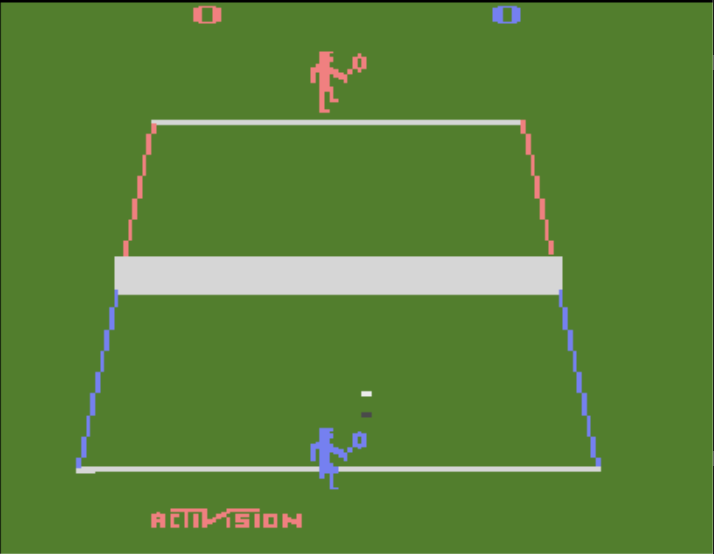
\includegraphics[width=0.45\textwidth]{image1.png} \caption{Przykładowy obraz ze środowiska} \label{fig:tennis} \end{figure}

\subsection{Opis Środowiska}
Bipedal Walker to środowisko należące do rodziny środowisk Box2D.  Przedstawia prostego robota kroczącego o czterech stawach (biodra i kolana) po terenie o niewielkich nierównościach. Wymaga sterowania ciągłego.

\subsection{Przestrzeń stanów (Observation Space)}

Stan środowiska opisuje wektor o 24 wymiarach, który zawiera:
\begin{itemize}
    \item kąt i prędkość kątową korpusu,
    \item prędkość poziomą i pionową,
    \item pozycje stawów oraz ich prędkości kątowe,
    \item informację o kontakcie nóg z podłożem,
    \item 10 pomiarów z lidarów (czujników odległości).
\end{itemize}
Wektor stanu nie zawiera współrzędnych absolutnych.





\subsubsection{Nagrody} 
Agent otrzymuje nagrodę za poruszanie się do przodu. Maksymalna suma nagród wynosi 300+ punktów, jeśli agent dotrze do końca terenu. Upadek robota powoduje karę w wysokości -100 punktów. Dodatkowo używanie momentu obrotowego silników kosztuje niewielką liczbę punktów.

\subsubsection{Stan początkowy}

Robot rozpoczyna symulację stojąc na lewej krawędzi terenu. Jego korpus jest ustawiony poziomo, a obie nogi znajdują się w identycznej pozycji z lekkim zgięciem kolan.

\subsubsection{Zakończenie epizodu}

Epizod kończy się w następujących sytuacjach:
\begin{itemize}
    \item korpus robota dotknie podłoża (upadek),
    \item robot przekroczy prawą krawędź terenu.
    \item Czas się skończy.
\end{itemize}
\subsubsection{Uruchomienie środowiska}
Aby zaimportować środowisko w języku Python, można skorzystać z poniższego fragmentu kodu: \begin{verbatim} env = gym.make("BipedalWalker-v3") \end{verbatim}


\section{Opis algorytmu Proximal Policy Optimization (PPO)}

\subsection{Teoretyczne podstawy algorytmu}
Proximal Policy Optimization (PPO) należy do klasy algorytmów uczenia ze wzmocnieniem opartych na optymalizacji strategii (policy optimization). Głównym celem algorytmu jest znalezienie optymalnej polityki \(\pi_\theta(a|s)\), która maksymalizuje skumulowaną wartość nagrody oczekiwanej:
\begin{equation}
J(\pi_\theta) = \mathbb{E}_{\pi_\theta} \left[ \sum_{t=0}^\infty \gamma^t r_t \right],
\end{equation}
gdzie:
\begin{itemize}
    \item \(\pi_\theta(a|s)\) – polityka parametryzowana przez \(\theta\), opisująca prawdopodobieństwo wyboru akcji \(a\) w stanie \(s\),
    \item \(\gamma\) – współczynnik dyskontowania, \(\gamma \in [0, 1]\),
    \item \(r_t\) – nagroda otrzymana w kroku \(t\).
\end{itemize}

PPO modyfikuje istniejącą politykę, aby poprawić jej skuteczność, ograniczając jednocześnie nadmierne zmiany w parametrach \(\theta\), co stabilizuje proces uczenia.

\subsection{Funkcja celu PPO}
Kluczowym elementem PPO jest funkcja celu (ang. \textit{clipped surrogate objective}). Funkcja ta opiera się na współczynniku prawdopodobieństwa:
\begin{equation}
r_t(\theta) = \frac{\pi_\theta(a_t | s_t)}{\pi_\text{old}(a_t | s_t)},
\end{equation}
gdzie \(\pi_\text{old}(a_t | s_t)\) to polityka przed aktualizacją parametrów.

Funkcja celu ogranicza zmiany w polityce za pomocą operatora \textit{clipping}:
\begin{equation}
L^\text{CLIP}(\theta) = \mathbb{E}_t \left[ \min \left( r_t(\theta) A_t, \text{clip}(r_t(\theta), 1 - \epsilon, 1 + \epsilon) A_t \right) \right],
\end{equation}
gdzie:
\begin{itemize}
    \item \(A_t\) – korzyść (ang. \textit{advantage}), która mierzy, jak korzystna jest dana akcja w stanie \(s_t\),
    \item \(\epsilon\) – parametr ograniczający zmiany w polityce, typowo \(\epsilon = 0.2\).
\end{itemize}

Dzięki tej funkcji algorytm unika zbyt dużych zmian w polityce, wybierając bardziej konserwatywne aktualizacje.

\subsection{Obliczanie korzyści (Advantage)}
PPO korzysta z metody Generalized Advantage Estimation (GAE) do obliczania korzyści \(A_t\):
\begin{equation}
A_t = \delta_t + (\gamma \lambda) \delta_{t+1} + (\gamma \lambda)^2 \delta_{t+2} + \ldots,
\end{equation}
gdzie:
\begin{equation}
\delta_t = r_t + \gamma V(s_{t+1}) - V(s_t).
\end{equation}

GAE pozwala kontrolować kompromis między wariancją a obciążeniem estymacji korzyści poprzez parametr \(\lambda \in [0, 1]\).

\subsection{Uczenie krytyka (Value Function Loss)}
Drugi komponent PPO to sieć krytyka, która uczy się wartości stanu \(V(s_t)\). Optymalizacja krytyka polega na minimalizacji błędu między przewidywaną wartością stanu a zwrotem (ang. \textit{return}):
\begin{equation}
L^\text{value}(\phi) = \mathbb{E}_t \left[ \max \left( (V_\phi(s_t) - R_t)^2, (V_\text{clip}(s_t) - R_t)^2 \right) \right],
\end{equation}
gdzie:
\begin{itemize}
    \item \(R_t = r_t + \gamma r_{t+1} + \gamma^2 r_{t+2} + \ldots\) – skumulowany zwrot,
    \item \(V_\text{clip}(s_t)\) – estymacja wartości stanu ograniczona do przedziału \([V_\text{old}(s_t) - \epsilon, V_\text{old}(s_t) + \epsilon]\).
\end{itemize}

\subsection{Regularizacja entropii}
Aby zachęcić agenta do eksplorowania środowiska, do funkcji celu PPO dodawany jest dodatkowy składnik związany z entropią polityki:
\begin{equation}
H(\pi_\theta) = -\sum_a \pi_\theta(a | s) \log \pi_\theta(a | s).
\end{equation}

Ostateczna funkcja celu PPO przyjmuje postać:
\begin{equation}
L(\theta) = L^\text{CLIP}(\theta) - c_1 L^\text{value}(\phi) + c_2 H(\pi_\theta),
\end{equation}
gdzie \(c_1\) i \(c_2\) to wagi regulujące wpływ poszczególnych składników.

\subsection{Proces treningu}
Proces treningu algorytmu PPO przebiega w następujących krokach:
\begin{enumerate}
    \item Agent zbiera doświadczenia w środowisku (stany, akcje, nagrody).
    \item Obliczane są zwroty \(R_t\) i korzyści \(A_t\).
    \item Aktualizowane są parametry:
    \begin{itemize}
        \item Polityki aktora poprzez maksymalizację \(L^\text{CLIP}(\theta)\),
        \item Sieci wartości poprzez minimalizację \(L^\text{value}(\phi)\).
    \end{itemize}
\end{enumerate}

\subsection{Podsumowanie}
Algorytm PPO to stabilna i skuteczna metoda optymalizacji polityki w uczeniu ze wzmocnieniem. Dzięki ograniczeniom wprowadzanym przez funkcję celu (clipping) oraz regularizacji entropii, PPO pozwala na efektywne uczenie się polityki przy zachowaniu stabilności. W projekcie algorytm został wykorzystany do sterowania agentem w środowisku \texttt{BipedalWalker-v3}.

\section{Opis drugiego algorytmu}

Ze względu na potencjalnie słabe wyniki standardowym podejściem Q-learning w złożonych środowiskach o ciągłej przestrzeni akcji, zastosowano ulepszoną architekturę modelu uczenia wzmocnionego wykorzystującą sieć Q z wieloma głowicami akcji oraz mechanizmem Double Q-Network. Poniżej przedstawiono podstawowe składniki tego modelu oraz sposób ich integracji.

\subsection{Q-Wartość (Q-Value)}

Q-wartość jest kluczowym pojęciem w uczeniu wzmocnionym. Reprezentuje ona oczekiwaną sumę nagród, jakie agent może uzyskać, wykonując określoną akcję w danym stanie środowiska i postępując zgodnie z określoną strategią. Formalnie:
\[
Q(s, a) = \text{oczekiwana suma nagród po wykonaniu akcji } a \text{ w stanie } s
\]

\subsection{Replay Buffer (Bufor Doświadczeń)}

Bufor Doświadczeń przechowuje doświadczenia agenta w postaci przejść \((s, a, r, s', done)\), gdzie:
\begin{itemize}
    \item \(s\) – obecny stan,
    \item \(a\) – wykonana akcja,
    \item \(r\) – otrzymana nagroda,
    \item \(s'\) – następny stan,
    \item \(done\) – flaga zakończenia epizodu.
\end{itemize}

Bufor umożliwia losowe próbkowanie mini-batchów doświadczeń do treningu, co pomaga w stabilizacji procesu uczenia poprzez redukcję korelacji między kolejnymi danymi treningowymi.

\subsection{Sieć Q (Q-Network)}

Sieć Q jest siecią neuronową, która przyjmuje stan środowiska jako wejście i przewiduje Q-wartości dla wszystkich możliwych akcji. W przedstawionym modelu:

\subsection{Double Q-Network Agent}

Agent zarządza procesem uczenia się, korzystając z dwóch sieci Q:
\begin{itemize}
    \item Główna sieć Q: Służy do przewidywania Q-wartości i podejmowania decyzji.
    \item Sieć docelowa Q: Używana do stabilizacji treningu poprzez dostarczanie stałych wartości docelowych, które są aktualizowane rzadziej.
\end{itemize}

\subsection{Strategia Eksploracji-Eksploatacji (Epsilon-Greedy)}

Strategia epsilon-greedy balansuje między eksploracją nowych akcji (wybór losowy) a eksploatacją znanych, najlepiej ocenianych akcji (wybór na podstawie sieci Q). Parametr \(\epsilon\) decyduje o prawdopodobieństwie wyboru akcji losowej.

\subsection{Opis Integracji}

Integracja podstawowych składników modelu odbywa się poprzez następujące kroki:

\begin{itemize}
    \item Interakcja z Środowiskiem:
    \begin{itemize}
        \item Agent rozpoczyna epizod, resetując środowisko i otrzymując początkowy stan \(s\).
    \end{itemize}
    
    \item Wybór Akcji:
    \begin{itemize}
        \item Na podstawie strategii epsilon-greedy, agent decyduje, czy wykonać akcję losową (eksploracja) czy wybrać akcję o najwyższej przewidywanej Q-wartości (eksploatacja) przy użyciu głównej sieci Q.
        \item W przypadku eksploatacji, sieć Q przetwarza stan \(s\) i generuje Q-wartości dla wszystkich możliwych akcji. Agent wybiera akcje z najwyższymi wartościami.
    \end{itemize}
    
    \item Wykonanie Akcji i Zbieranie Doświadczeń:
    \begin{itemize}
        \item Wybrana akcja \(a\) jest wykonana w środowisku, co skutkuje przejściem do nowego stanu \(s'\), otrzymaniem nagrody \(r\) oraz informacją o zakończeniu epizodu (\(done\)).
        \item Przejście \((s, a, r, s', done)\) jest dodawane do Replay Buffer.
    \end{itemize}
    
    \item Próbkowanie i Trening Sieci Q:
    \begin{itemize}
        \item Gdy Replay Buffer jest wystarczająco pełny (np. więcej niż 5000 przechowywanych przejść), agent losowo wybiera mini-batch doświadczeń do treningu.
        \item Sieć Q przetwarza stany \(s\) z mini-batcha, przewidując obecne Q-wartości dla wykonanych akcji.
        \item Sieć docelowa Q przetwarza następne stany \(s'\), przewidując przyszłe Q-wartości. Używa się ich do obliczenia wartości docelowych:
        \[
        \text{target} = r + \gamma \cdot \max_{a'} Q_{\text{target}}(s', a') \cdot (1 - done)
        \]
        \item Funkcja straty (średniokwadratowy błąd) porównuje obecne Q-wartości z wartościami docelowymi.
        \item Optymalizator (Adam) aktualizuje wagi głównej sieci Q na podstawie obliczonych gradientów.
    \end{itemize}
    
    \item Aktualizacja Sieci Docelowej:
    \begin{itemize}
        \item Co określoną liczbę kroków, wagi sieci docelowej są synchronizowane z wagami głównej sieci Q, co pomaga w stabilizacji procesu uczenia.
    \end{itemize}

\end{itemize}









\section{Trenowanie Modeli RL}
W celu porównania skuteczności modeli przeanalizowaliśmy nagrodę uzyskiwaną na epizod. Wynik działania poszczególnych modeli zamieszczony w osobnych plikach.


\begin{figure}[htbp]
    \centering
    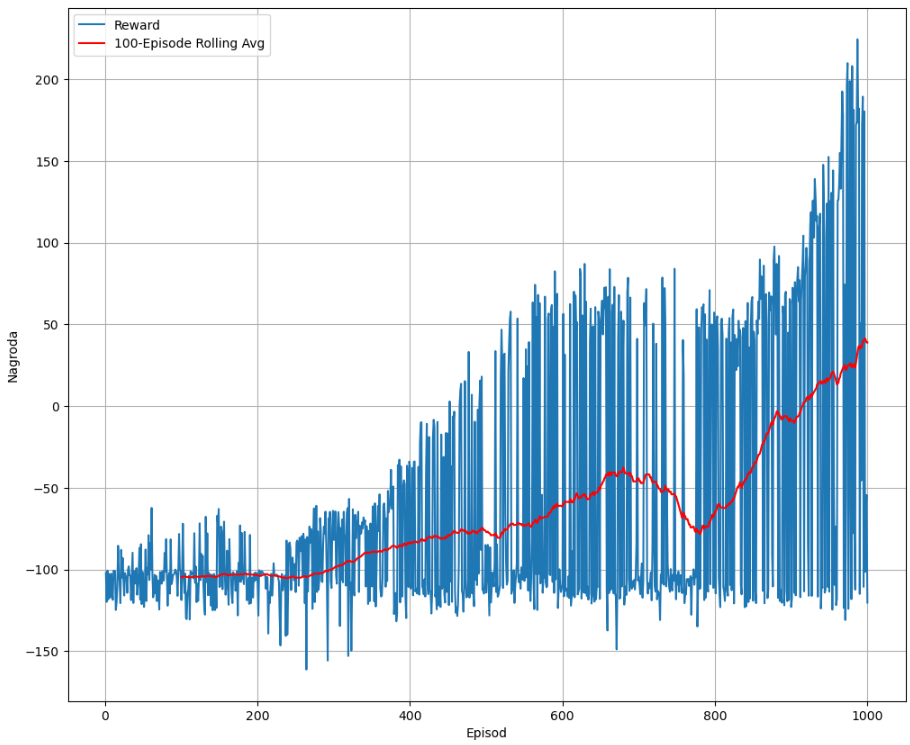
\includegraphics[width=0.45\textwidth]{image2.png}
    \caption{Trening model 1 PPO}
    \label{fig:ppo}
\end{figure}


\begin{figure}[htbp]
    \centering
    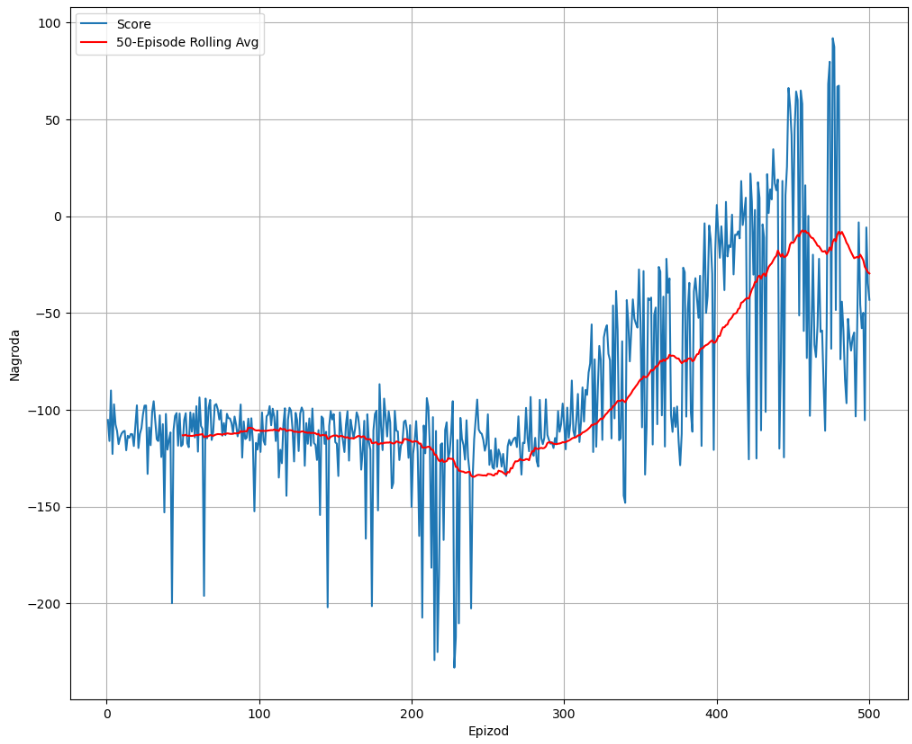
\includegraphics[width=0.45\textwidth]{image3.png}
    \caption{Trening model 2 value based}
    \label{fig:dqn}
\end{figure}






\section{Wnioski}
\begin{itemize}
    \item Oba zastosowane modele uczenia przez wzmacnianie, Proximal Policy Optimization (PPO) oraz wariancja DQN, pozwoliły na wytrenowanie relatywnie satysfakcjonującego wytrenowany model.
    
    \item Algorytm PPO osiągnął lepsze wyniki w porównaniu do DQN oraz jego czas nauki był o wiele krótszy, co nie zostało uwzględnione w wykresach i statystykach raportu, ale jest istotnym aspektem efektywności algorytmu.   
    
    \item Ze względu na to że tradycjne podejścia value-based były potencjalnie nieefetywne przetestowano modyfikacje, mimo to i tak dały wyniki gorsze od metody policy based.
\end{itemize}





\end{document}